% Пусть $f\!: \R^1 \to \R^1$. Тогда можно определить $\Delta f = A \Delta x + \overline{\overline{o}}(\Delta x)$, где $A = f'(x_0)$.
% не будем в этом параграфе отвлекаться на комплексности

% метрическое пространство придумали между титаником и пулеметом максим
\begin{definition}
    Пусть $E_1, E_2$~--- вещественные банаховы пространства. $D \subset E_1$~--- область, $F\!: D \to E_2$~--- отображение. $F$ называется \textit{дифференцируемым по Фреше} в точке $x_0$, 
    если \newline  $\exists A \in \L(E_1, E_2)$ такой, что $\Delta F = F(x_0 + h) - F(x_0) = A h + \varepsilon(h)$, где $\frac{\|\varepsilon(h) \|}{\|h\|} \xrightarrow[h \to 0]{} 0$. \newline $A$ называют производной Фреше, $A = F'(x_0)$
\end{definition}

\begin{definition}
    \textit{Дифференциалом Фреше} в точке $x_0$ на приращение $h$ называется 
    $dF(x_0, h) = F'(x_0) h$. При этом $F' \in \L(E_1, E_2), h \in E_1$, а итог $\in E_2$.
\end{definition}

\begin{lemmanote}
    Производная~--- это оператор, дифференциал~--- это значение этого оператора на аргументе приращения.
\end{lemmanote}
% дуэль Коновалова и Редкозубова

\begin{definition}[эквивалентное определение]
    \[
    \frac{\|\Delta F - Ah\|}{\|h\|} \xrightarrow[h \to 0]{} 0
    \]
\end{definition}

\begin{statement}\(\)
    \begin{enumerate}
        \item[0.]  Дифференцируемость по Фреше влечёт непрерывность в точке.
        \item[1.] Если $\forall x \in D\:F(x) = \text{const} (\in E_2)$, то $\forall x \in D \: F'(x) = 0$.
        \item[2.] Если $F \in \L(E_1,E_2)$, то $\forall x \in E_1 \; F'(x)=F$
        \item[3.] $(\alpha_1 F_1 + \alpha_2 F_2)'=\alpha_1 F_1' + \alpha_2 F_2'$
        \item[4.] $F\!\!: E_1 \to E_2, \; G\!\!: E_2 \to E_3$~--- дифференцируемы. 
        Тогда $H = G \circ F$ дифференцируема и $H' = G' \circ F'$. (док-во \ref{Freshe-diff-4})
    \end{enumerate}
\end{statement}

% ГОСТ 7.0.12-2011 Правильно сокращать дифференцируемость как диф., а не дифф. Но мы будем не по ГОСТу

\begin{definition}
    $F\!: D \to E_2$. Если существует \[DF(x_0; h) = \frac{d}{dt} F(x_0 + th) \Big|_{t = 0} = \lim\limits_{\R \ni t \to 0} t^{-1}\left(F(x_0 + th) - F(x_0)\right),\] то говорим, что определен \textit{дифференциал Гато}. А если 
    $DF(x_0; h) = Ah$, где $A = F'_{\text{сл.}}(x_0)$ называется \textit{слабой производной Гато}.
\end{definition}
\begin{statement}
    \begin{itemize}
        \item[] 
        \item[1.] Дифф-ть по Фреше $\implies$ дифф-ть по Гато и $F'_{\text{сл.}}=F'_{\text{Фр.}}$.
        \item[2.] В обратную сторону это неверно
        \begin{figure}[H]
            \centering
            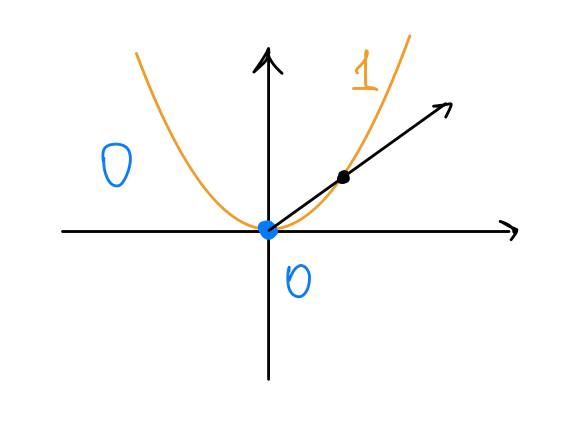
\includegraphics[width=0.25\textwidth]{images/dF_parabola.jpg}
        \end{figure}
        На картинке изображена функция $f\!\!: \R^2 \to \R$ такая, что на параболе единица, на всем остальном ноль. 
        
        Очевидно, что производная по всем направлениям в нуле одинаковая и нулевая, но она есть. А вот по Фреше производной нет~--- функция даже не непрерывна в $(0; 0)$.
    \end{itemize}
\end{statement}

\begin{unnecessary}
    \begin{example}
    В пространстве $C[a,b]$
    \[
    (Af)(x) = \int_a^b K(x, t, f(t)) dt
    \]
    
    \[
    \frac{d}{dx} \int_a^b K(x, t, f(t)) dt
    \]
    Когда дифференцирование и интеграл можно переставить местами?
    \end{example}
    
    \begin{exercise}
        $H(\R), f(x)=\|x\|$. Где он дифференцируем? (ответ: везде кроме 0)
    \end{exercise}
\end{unnecessary}






\begin{theorem}[13.1 (формула конечных приращений)]\label{13.1}
% название не устоявшееся
Пусть $E_1, E_2$~--- вещественные банаховы пространства,  $D$~-- выпуклая область, $F\!: D \to E_2$~--- дифференцируема по Фреше. \newline
Тогда $\forall x_0, x_1 \in D$
\[
\|F(x_1) - F(x_0)\| \leqslant \sup_{y \in (x_0, x_1)}
\|F'(y)\| \cdot \|x_1 - x_0\|
\]
\end{theorem}

\begin{proof}
\begin{figure}[H]
    \centering
    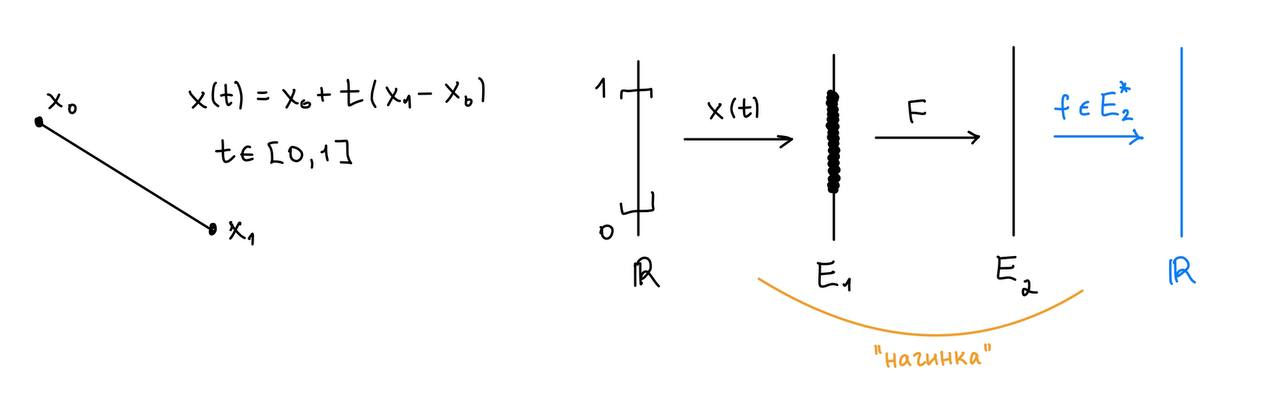
\includegraphics[width=0.7\textwidth]{images/sandwich.jpg}
\end{figure}
Возьмём $f \in E_2^*$ и введем функцию $\varphi(t) = f(F(x(t)))$ дифференцируема, так как $f$~--- это линейный непрерывный функционал, а значит имеет производную в каждой точке, совпадающую с самим этим функционалом, $F$ дифференцируем по Фреше по условию, а $x(t)$ видно по формуле, что дифференцируема.

\[
\varphi(1) - \varphi(0) = f(F(x_1)) - f(F(x_0)) = 
f(F(x_1) - F(x_0))
\]

\[
    \varphi'(t)=f(F'(x(t))(x_1-x_0))
\]

$f$ не затронута операцией дифференцирования, так как является линейным функционалом.

Воспользуемся следствием \nameref{hbcorollary2} из теоремы Хана-Банаха:
$E$~--- НП, $0 \neq x \in E$.
Тогда $\exists f \in E^*$, такой что $\|f\| = 1$ и $f(x) = \|x\|$.

Возьмём такой $f \in E_2^*$ для $\Big(F(x_1)-F(x_0)\Big) \in E_2$. Для этого $f$
\[
\varphi(1) - \varphi(0) = \|F(x_1) - F(x_0)\|
\]

По обычной теореме Лагранжа \[\exists \xi \in (0; 1)\: |\varphi'(\xi)(1-0)|=|\varphi(1)-\varphi(0)| \]

\[
|f(F'(x_{\xi}) \underbrace{(x_1 - x_0)}_{\Delta x})| \leqslant \underbrace{\|f\|}_{1} \cdot
\sup_{y \in (x_0, x_1)} \|F'(y)\| \cdot \|x_1 - x_0\|
\]

\end{proof}

\begin{exercise}
    Придумать пример $F, G$~--- слабо дифференцируемы, а $H=G \circ F$~--- нет
\end{exercise}

\begin{theorem}[13.2]
    $F'_{\text{сл.}}(x_0)$ существует и непрерывна в окрестности $x_0 \implies \exists F'_{\text{Фр.}}(x_0)=F'_{\text{сл.}}(x_0)$ 
\end{theorem}

\begin{statement}[(одно из свойств)]
    Если $F, G$~--- дифференцируемы по Фреше, то $H=G \circ F$~--- дифференцируема по Фреше и $H'(x_0)= (G' \circ F')(x_0)$
\end{statement}

\begin{unnecessary}
    \textbf{Применение теоремы \nameref{13.1}:}
    \begin{enumerate}
        \item Дифференциальное исчисления в банаховых пространствах.
        В частности, решение экстремальных задач.
        % книжка Иоффе, Тихомиров, Экстремальные задачи 1974
        Вариационное исчисление: вариация по Лагранжу $==$ слабый дифференциал Гато
    
        \item Решение уравнений, метод Ньютона,...
        Таким образом, Теорема \nameref{13.1}~--- это удобный способ установления того, что $F$~--- сжимающее отображение.
        В частности: решение уравнений $F(x)=0$ ($x_{n+1}=x_n-[F'(x_n)]^{-1} F(x_n)$. Если предел существует, то $x=x-[F'(x)]^{-1} F(x)$, то есть $F(x)$ должен равняться 0)
        % книжка Канторович, Акилов, Функциональный анализ, Часть II: "Функциональные уравнения"
    \end{enumerate}
\end{unnecessary}


\begin{statement}\label{Freshe-diff-4}
    $F: X \to Y$ дифференцируема в точке $x_0$, $G: Y \to Z$ дифференцируема в точке $y_0 = F x_0$. Тогда $H = G \circ F$ дифференцируема в точке $x_0$.
\end{statement}
% картинка 1
\begin{proof}
        % развинчиваем внешнюю матрешку
        \[ \Delta z = G'(y_0) \Delta y + \varepsilon_1(\Delta y) \text{, где } \frac{\|\varepsilon_1(\Delta y)\|_Z}{\|\Delta y \|} \to 0 \]

        \[
        \Delta y = F'(x_0) \Delta x + \varepsilon_2(\Delta x)
        \]

        Хитро подставим $\Delta y$ в выражение для $\Delta z$

        \[ 
        \Delta z = G'(y_0)\Big(F'(x_0) \Delta x + \varepsilon_2(\Delta x)\Big) + \varepsilon_1(\Delta y)=G'(y_0) \circ F'(x_0) \Delta x + G'(y_0) \varepsilon_2(\Delta x) + \varepsilon_1(\Delta y)
        \]

        Хотим, чтобы $G'(y_0) \varepsilon_2(\Delta x) = \overline{\overline{o}}(\Delta x)$ при $\Delta x \to 0$.
        \[
        \frac{\|G'(y_0) \varepsilon_2(\Delta x)\|}{\|\Delta x\|}
        \leqslant \frac{\|G'(y_0)\| \cdot \|\varepsilon_2(\Delta x)\|}{\|\Delta x\|} \to 0,
        \]
        так как $\frac{\| \varepsilon_2(\Delta x) \|_Y}{\| \Delta x \|} \xrightarrow[\Delta x \to 0]{} 0$.
        
        Надо показать, что $\|\varepsilon_1(\Delta y)\| = \overline{\overline{o}}(\|\Delta x\|)$ 

        \[
        \frac{\|\varepsilon_1(\Delta y)\|}{\|\Delta x\|} \cdot \frac{\|\Delta y\|}{\|\Delta y\|}
        \]
        
        Тут <<главная диагональ>> в пределе даёт 0 при $\|\Delta x \| \to 0$ и $\|\Delta y \| \to 0$ (см. первую строку доказательства)
        
        \[
        \frac{\|\Delta y\|}{\|\Delta x\|} = 
        \frac{\|F'(x_0) \Delta x + \varepsilon_2(\Delta x)\|}{\|\Delta x\|} \leqslant 
        \frac{\|F'(x_0)\| \cdot \|\Delta x\| + \|\varepsilon_2(\Delta x)\|}{\|\Delta x\|} \leq \text{const}
        \]

        Т.е <<побочная диагональ>> ограничена и домножается на <<главную диагональ>>, которая стремиться к нулю. Значит, и все выражение стремится к нулю.
\end{proof}

